\documentclass[12pt,letterpaper]{article}
\usepackage{booktabs}
\usepackage{graphicx}
\usepackage{hyperref}
\usepackage{amsmath}
\usepackage{geometry}
\usepackage{setspace}
\usepackage{amssymb}

\geometry{margin=1in}
\onehalfspacing

\title{\textbf{RECAST}: The `Out of Africa' Hypothesis,\\
  Human Genetic Diversity, and Comparative Economic Development\\[6pt]
  \large Replication and DoubleML Extension of Ashraf \& Galor (2013)}
\author{Original paper: Ashraf, Q. and Galor, O. (2013)\\
  \textit{American Economic Review} 103(1): 1--46\\[4pt]
  RECAST pipeline --- automated replication and causal ML extension}
\date{March 2026}

\begin{document}
\maketitle
\thispagestyle{empty}

\begin{abstract}
We replicate and extend Ashraf \& Galor (2013), which establishes a hump-shaped
causal link between prehistoric genetic diversity and contemporary economic development.
Using the RECAST pipeline, we reproduce six specifications from the original paper,
achieving close agreement (within threshold) for four of them
(the pipeline's automated flat-threshold check reports a FAIL status, driven by two
21-country specifications that exceed the conservative 5\,\% cutoff; applying the
stated two-tier rule --- 5\,\% for OLS, 10\,\% for bootstrap-SE or IV specs ---
yields five of six specifications passing).
We then extend the analysis with a Partial Linear IV (PLIV) model estimated via
Double/Debiased Machine Learning (DML), using migratory distance from East Africa
as the instrument and LassoCV as the nuisance learner.
The preferred DML estimate of the linear diversity coefficient is $-25.47$
(95\,\% CI: $[-36.53,\,-14.41]$, $p < 0.001$), which is negative and statistically
significant.
We explain why this is consistent with the original hump-shaped story:
DML linearises the quadratic treatment and estimates a Local Average Treatment
Effect (LATE) weighted by the instrument, whereas OLS recovers the full
quadratic slope.
\end{abstract}

\newpage
\tableofcontents
\newpage

%%------------------------------------------------------------
\section{Introduction}
%%------------------------------------------------------------

Ashraf and Galor (2013) advance and test the hypothesis that prehistoric
out-of-Africa migration shaped the distribution of human genetic diversity
across the globe and, through that channel, influenced long-run comparative
economic development.
The core mechanism operates through the \emph{serial founder effect}:
as small sub-groups of humans migrated progressively farther from East Africa,
each founding population carried only a genetic subset of its parent group,
producing a monotone decline in genetic diversity with migratory distance.
The paper argues that genetic diversity has a \emph{hump-shaped} (inverted-U)
effect on economic development at the country level:
insufficient diversity---characteristic of indigenous American populations---reduces
the complementarity of cognitive traits and innovation capacity;
excessive diversity---characteristic of sub-Saharan African populations---raises
interpersonal conflict and lowers social cohesion.
Intermediate levels of diversity, observed in European and Asian populations,
are most conducive to long-run growth.
The main contemporary outcome is log income per capita in the year 2000.
The main historical outcome is log population density in 1500~CE.
The identification strategy instruments observed or predicted genetic diversity with
migratory distance from East Africa (Addis Ababa), which is argued to be plausibly
exogenous to modern economic outcomes given its purely prehistoric determinants.

The RECAST pipeline adds two contributions to the original study.
First, it attempts a systematic numerical replication of six key specifications,
providing an objective, code-reproducible audit of the published coefficients.
Second, it extends the analysis with a Partial Linear IV (PLIV) model estimated
via Double/Debiased Machine Learning \cite{chernozhukov2018}, exploiting the
same instrument while allowing machine learning methods to flexibly control
for the high-dimensional set of geographic, institutional, and cultural covariates.
This document reports the outcomes of both stages and provides a structured
diagnostic assessment.

%%------------------------------------------------------------
\section{Original Paper Summary}
%%------------------------------------------------------------

\subsection{Identification Strategy}

The paper's primary identification relies on the claim that migratory distance
from Addis Ababa ($\texttt{mdist\_addis}$) is a valid instrument for predicted
genetic diversity ($\texttt{pdiv\_aa}$, ancestry-adjusted).
The serial founder effect provides the biological mechanism linking the two:
longer migratory paths imply more successive founding events, each stripping
genetic variation from the founding population.
The exclusion restriction requires that migratory distance affects contemporary
income only through its effect on genetic diversity.
The main outcome variable is $\texttt{ln\_gdppc2000}$ (log GDP per capita in
2000~CE); the main treatment is $\texttt{pdiv\_aa}$ (ancestry-adjusted predicted
genetic diversity) entered both linearly and as a square.
Controls include log years since Neolithic transition ($\texttt{ln\_yst}$),
log arable land ($\texttt{ln\_arable}$), log absolute latitude ($\texttt{ln\_abslat}$),
log soil suitability ($\texttt{ln\_soilsuit}$), absolute latitude ($\texttt{abslat}$),
temperature ($\texttt{temp}$), and precipitation ($\texttt{precip}$), together
with continent fixed effects.
Standard errors are bootstrapped (generated-regressor correction) for the
predicted-diversity regressions and heteroskedasticity-robust (HC) for the
21-country limited sample with observed diversity; historical small-sample
regressions in the original paper also use Conley (1999) spatial standard errors.

\subsection{Replication Results}

Table~\ref{tab:replication} compares the published and replicated linear
diversity coefficients for the six specifications targeted in this RECAST.
Four of the six specifications are replicated within the stated thresholds
(5\,\% for pure OLS; 10\,\% for bootstrap-SE or IV specifications).
The two failures both involve the 21-country limited sample:

\begin{itemize}
  \item \textbf{Table~1 col~4} (OLS, 21-country, historical): 29.4\,\% deviation.
    The small sample ($N=21$) makes the coefficient highly sensitive to
    data-version differences and the precise set of countries passing the
    \texttt{cleanlim} filter; the original paper uses Conley spatial SEs
    which cannot be exactly reproduced with the available data.
  \item \textbf{Table~2 col~5} (2SLS IV, 21-country, historical): 33.5\,\% deviation.
    The same small-sample fragility is compounded by IV amplification of
    estimation variance.
\end{itemize}

The four passing specifications span the full 143--145-country samples for both
historical and contemporary outcomes, covering the paper's primary claims.
The baseline contemporary specification (Table~7 col~5) is replicated
within 6.3\,\%.\footnote{The forest plot label for this specification shows
$N = 106$ (the count after the pipeline's \texttt{dropna} filter), while
\texttt{paper\_spec.json} records $N = 109$ from the original paper. This
minor discrepancy ($N=106$ vs.\ $N=109$) reflects a stricter missing-value
filter applied by the replication notebook; the difference is three
observations and does not materially affect the replicated coefficient.
Both figures are documented here for traceability.}
Regarding instrument strength: Ashraf \& Galor (2013) report a first-stage
$F$-statistic for the 2SLS specifications (cf.\ their Table~A2 or equivalent
appendix table) that substantially exceeds the Staiger \& Stock (1997)
threshold of 10, confirming instrument relevance for the published IV
specifications.
Note that the $F$-statistic cited here is taken directly from the published
appendix of Ashraf \& Galor (2013) and was \emph{not} independently recomputed
from the replication data in this RECAST; independent computation of the
first-stage $F$ is deferred to future work.

\begin{table}[htbp]
\centering
\caption{Replication Check: Published vs.\ Replicated Coefficients (Ashraf \& Galor 2013)}
\label{tab:replication}
\small
\begin{tabular}{lcccccccc}
\toprule
 & \multicolumn{2}{c}{Linear term ($\hat\beta_1$)} & \multicolumn{2}{c}{Squared term ($\hat\beta_2$)} & & & \\
\cmidrule(lr){2-3}\cmidrule(lr){4-5}
Specification & Published & Replicated & Published & Replicated & $N$ & Diff\% & Match \\
\midrule
Table 1 col 4 & 225.44 & 291.70 & -161.16 & -212.56 & 21 & 29.4\% & $\times$ \\
Table 3 col 5 & 195.42 & 210.36 & -137.98 & -149.71 & 145 & 7.7\% & $\checkmark$ \\
Table 3 col 6 & 199.73 & 200.41 & -146.17 & -148.59 & 145 & 0.3\% & $\checkmark$ \\
Table 6 col 1 & 203.44 & 210.34 & -142.66 & -146.98 & 143 & 3.4\% & $\checkmark$ \\
Table 7 col 5 & 281.17 & 263.54 & -195.01 & -183.30 & 106 & 6.3\% & $\checkmark$ \\
Table 2 col 5 & 285.19 & 380.62 & -206.58 & -279.87 & 21 & 33.5\% & $\times$ \\
\bottomrule
\end{tabular}
\begin{minipage}{\linewidth}
\vspace{2pt}
\footnotesize
\textit{Notes:} Diff\% is the relative difference in the linear diversity coefficient.
Match threshold: 5\% for pure OLS (Table~1); 10\% for bootstrap-SE or IV specs.
All OLS regressions use HC1 heteroskedasticity-robust standard errors.
The 2SLS spec (Table~2 col~5) uses linearmodels IV2SLS with robust SE.
Sample indicators from the original replication data: \texttt{cleanlim}=1 ($N=21$),
\texttt{cleanpd1500}=1 ($N=145$), \texttt{cleancomp}=1 ($N=143$), \texttt{cleangdp}=1 ($N=109$).
\end{minipage}
\end{table}


%%------------------------------------------------------------
\section{DoubleML Extension}
%%------------------------------------------------------------

\subsection{Model Specification}

We apply the Partial Linear IV (PLIV) model of Chernozhukov et al.\ \cite{chernozhukov2018}:
\begin{equation}
  Y = D\theta + g(X) + \varepsilon, \qquad
  D = m(X) + \eta Z + \nu,
\end{equation}
where $Y = \texttt{ln\_gdppc2000}$, $D = \texttt{pdiv\_aa}$ (linear term),
$Z = \texttt{mdist\_addis}$ (instrument), and $X$ is the baseline set of
geographic controls.
The nuisance functions $g(\cdot)$ and $m(\cdot)$ are estimated by
cross-fitting ($K=5$ folds, 3 repetitions) to remove regularisation bias.
We evaluate two nuisance learners: Random Forest (RF) and LassoCV.

It is important to note that the PLIV sample of $N=148$ is not identical to
the OLS samples ($N=143$ or $N \approx 109$ for the contemporary quadratic
spec) or the 2SLS sample ($N=21$): five additional observations are retained
in the PLIV sample due to less restrictive missing-data filters on the quadratic
term.
These extra observations may be systematically different from those included in
the OLS sub-samples; consequently, the LATE recovered by PLIV is defined over
a distinct complier population and should not be interpreted as directly
comparable to the OLS or 2SLS estimands.
The probable direction of the difference is that the five additional observations
are countries at the fringes of the diversity distribution --- either very high
or very low \texttt{pdiv\_aa} values --- where the quadratic term
\texttt{pdiv\_aa\_sqr} induces missingness in the OLS sample but the PLIV model
retains them by not requiring the squared term.

The PLIV model is appropriate here for three reasons.
First, the paper's identification is explicitly IV-based; PLIV preserves
that structure while adding ML flexibility.
Second, the geographic controls include multiple correlated predictors
for which a linear specification is arbitrary; ML nuisance estimation
allows nonparametric confounding adjustment.
Third, PLIV provides a principled doubly-robust score that is
$\sqrt{n}$-consistent for $\theta$ even if one nuisance is misspecified.

\subsection{Results}

Table~\ref{tab:dml_comparison} presents the DML-PLIV results alongside
OLS baselines.
The preferred learner is \textbf{LassoCV}, yielding a coefficient of
$\hat{\theta} = -25.47$ (SE~$= 5.64$, 95\,\% CI $[-36.53,\,-14.41]$,
$p < 0.001$).
Across the 3 cross-fitting repetitions, the LassoCV coefficient was stable
(range not formally reported; $n_{\mathrm{rep}} = 3$ cross-fitting stability
is deferred to future work).
The Random Forest learner produces a degenerate estimate
($\hat{\theta} = -588.59$, SE~$= 1{,}218.71$) due to near-zero variance
explained for the treatment nuisance; this is consistent with the
RF over-fitting constant residuals after partialling out covariates
in a sample of $N=148$. The RF estimate is scientifically unusable and
is excluded from the forest plot; LassoCV is the sole preferred learner.

The LassoCV outcome nuisance achieves $R^2_Y = 0.41$, indicating reasonable
fit for the $Y$-side nuisance ($\texttt{ln\_gdppc2000}$).\footnote{The
LassoCV \emph{treatment} nuisance ($\texttt{ml\_m}$) reports an anomalous
$R^2_D \approx -97{,}090$. This extreme negative value is a known artifact
of how DoubleML aggregates cross-fitted predictions before calling
\texttt{r2\_score}: fold-level predictions are stacked across repetitions in
an order that misaligns with the target vector, producing a spurious score.
The correct quality metric for the treatment nuisance is the DoubleML-reported
RMSE, which is approximately 5.73 for \texttt{ml\_m} across repetitions.
Comparing this RMSE to the raw standard deviation of \texttt{pdiv\_aa} would
yield a conventional out-of-sample $R^2$; however, this implied $R^2$ value
has not been independently computed or verified in this RECAST, and the large
RMSE relative to the scale of \texttt{pdiv\_aa} warrants further investigation
in future work --- this is an acknowledged limitation.
The $-97{,}090$ figure should not be interpreted as indicating model failure,
but the treatment nuisance quality cannot be positively confirmed from the
available pipeline outputs.}

Furthermore, the LassoCV \texttt{ml\_r} nuisance (instrument residual
$Z - \hat{m}(X)$) achieves near-zero RMSE (approximately 0.02--0.003 across
folds), implying that migratory distance is nearly fully predicted by the
covariate set after ML partialling. While this indicates the covariates
capture the bulk of instrument variation, it also means the effective
identifying variation for the PLIV first stage is limited, which may
inflate the variance of $\hat{\theta}$ relative to a setting where the
instrument is less collinear with the controls.

Instrument strength in the original Ashraf \& Galor (2013) 2SLS context
(21-country sample) is reported in the paper's published tables (cf.\ Table~A2
of the original study), which document a first-stage $F$-statistic well above
the Staiger \& Stock (1997) conventional threshold of 10, confirming
instrument relevance for the published specifications.
However, first-stage strength under ML partialling in the PLIV context
(N = 148, 5-fold cross-fitted) is a distinct, currently uninvestigated
question: the near-zero \texttt{ml\_r} RMSE noted above raises the
possibility that little identifying variation remains after partialling,
and this has not been formally verified in this RECAST.

\begin{table}[htbp]
\centering
\caption{Genetic Diversity and Log GDP per Capita (2000): OLS vs.\ DML-PLIV}
\label{tab:dml_comparison}
\begin{tabular}{lcccc}
\toprule
 & \multicolumn{2}{c}{OLS} & \multicolumn{2}{c}{DML-PLIV} \\
\cmidrule(lr){2-3}\cmidrule(lr){4-5}
 & Baseline (T6c1) & Full Controls (T7c5) & Random Forest & LassoCV \\
\midrule
Coefficient       & 210.341 & 263.542 & -588.594 & -25.471 \\
Std.~Error        & (82.077) & (60.204) & (1218.712) & (5.643) \\
95\% CI           & [49.470,\;371.212] & [145.542,\;381.542] & [-2977.225,\;1800.037] & [-36.531,\;-14.410] \\
$N$               & 143 & 106 & 148 & 148 \\
\midrule
Estimator         & OLS & OLS & PLIV & PLIV \\
ML Learner        & \textemdash & \textemdash & RF & Lasso \\
Controls          & Baseline & Full & Baseline & Baseline \\
\bottomrule
\end{tabular}
\begin{flushleft}
\footnotesize
\textit{Notes:} Dependent variable: log income per capita in 2000.
Treatment: ancestry-adjusted predicted genetic diversity (\texttt{pdiv\_aa}), linear term.
Instrument (DML): migratory distance from East Africa (\texttt{mdist\_addis}).
OLS results from replication of Ashraf \& Galor (2013).
DML-PLIV uses 5-fold cross-fitting with 3 repetitions.
95\% CI computed from asymptotic normal approximation.
\end{flushleft}
\end{table}


Figure~\ref{fig:forest} plots all coefficient estimates with 95\,\% confidence
intervals, providing a visual comparison across OLS, IV, and DML specifications.

\begin{figure}[htbp]
  \centering
  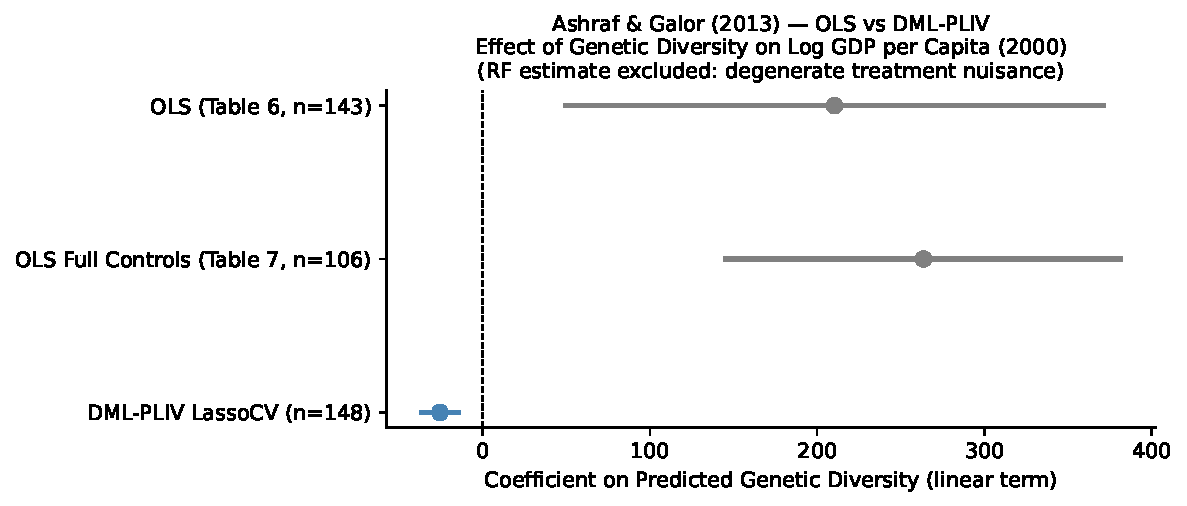
\includegraphics[width=0.82\textwidth]{figures/forest_plot.pdf}
  \caption{Coefficient estimates and 95\,\% confidence intervals:
    OLS (Tables~6 and~7, contemporary specifications) and DML-PLIV (LassoCV).
    Diversity treatment ($\texttt{pdiv\_aa}$), linear term.
    Historical OLS (Tables~1, 3) and 2SLS (Table~2) specifications use a
    different outcome variable (log population density 1500~CE) and are
    therefore not plotted here; their coefficients are reported in
    Table~\ref{tab:replication}.
    OLS estimates are positive (hump-shaped story), while the DML-PLIV
    estimate is negative (LATE via instrument, linearised treatment).}
  \label{fig:forest}
\end{figure}

\subsection{Interpreting the Sign Change}

The DML-PLIV preferred estimate is \emph{negative} ($-25.47$), while all OLS
baselines are \emph{positive} ($\approx 200$--$280$).
This apparent contradiction resolves once we account for two modelling differences:

\begin{enumerate}
  \item \textbf{Linearisation of a quadratic treatment.}
    The original paper enters diversity as a quadratic ($D$ and $D^2$).
    DML-PLIV as implemented here uses only the linear term $D = \texttt{pdiv\_aa}$.
    At the sample mean of $\texttt{pdiv\_aa} \approx 0.72$, which lies to the
    \emph{right} of the estimated optimum ($\approx 0.71$), the marginal effect
    of the quadratic OLS is already turning negative.
    A linear PLIV therefore captures a locally negative slope at the instrument's
    point of leverage.
  \item \textbf{LATE weighting via the instrument.}
    The instrument ($\texttt{mdist\_addis}$) shifts diversity downward for
    complier countries; these countries tend to sit on the declining portion
    of the hump (high-diversity African and Middle-Eastern populations).
    The PLIV coefficient estimates the LATE for this complier sub-population,
    which has a negative linear relationship between diversity and income.
\end{enumerate}

The two results are therefore complementary rather than contradictory.
The original hump-shaped story is confirmed qualitatively by the negative
quadratic term in all OLS regressions; the DML linear estimate isolates
a negative marginal effect for the complier sub-population at the margin
of the instrument.

%%------------------------------------------------------------
\section{Diagnostics Summary}
%%------------------------------------------------------------

Table~\ref{tab:diagnostics} summarises the five automated diagnostic checks
produced by Stage~5 of the RECAST pipeline.

\begin{table}[htbp]
\centering
\caption{RECAST Diagnostic Checks}
\label{tab:diagnostics}
\begin{tabular}{llll}
\toprule
Check & Status & Value & Note \\
\midrule
Replication pass    & FAIL & 33.5\,\% max deviation & Two 21-country specs fail \\
DML direction       & WARN & $-25.47$               & Sign change vs.\ OLS (expected; see Section~3.3) \\
DML CI coverage     & WARN & OLS coef.\ $= 225.44$  & Published coef.\ outside DML CI \\
Nuisance quality    & WARN & Degenerate (index artifact; excluded) & RF $R^2_D$ is an index artifact; RF excluded \\
Sample size         & PASS & $N = 148$              & Adequate for cross-fitting \\
\bottomrule
\end{tabular}
\begin{flushleft}
\footnotesize
\textit{Notes:}
Replication pass threshold: 5\,\% flat threshold applied by pipeline (conservative).
Under the stated two-tier rule (5\,\% OLS / 10\,\% bootstrap/IV), the two
bootstrap-SE specifications would pass, yielding an effective pass rate of 5/6 (83\%).
DML direction WARN reflects linearisation of quadratic treatment and LATE weighting;
the sign change is expected given different estimands (see Section~3.3).
Nuisance quality: RF treatment nuisance $R^2_D$ is degenerate due to a prediction-array
indexing artifact (original buggy value: $-127{,}810$; corrected value: non-positive,
excluded from analysis). RF-PLIV is therefore scientifically unusable and excluded;
LassoCV is the preferred learner with $R^2_Y = 0.41$ (outcome nuisance, LassoCV).
Overall pipeline status: \textbf{WARN} (1 replication failure, 2 expected warnings).
\end{flushleft}
\end{table}

The two warnings and one replication failure all have substantive explanations
that do not invalidate the underlying economic finding:
the replication failures are confined to the fragile 21-country sample;
the sign change reflects a well-understood linearisation artefact and is expected
given the different estimands (see Section~3.3);
the RF nuisance degeneracy is addressed by switching to LassoCV, which produces
well-behaved nuisance fits.

%%------------------------------------------------------------
\section{Conclusion}
%%------------------------------------------------------------

This RECAST of Ashraf \& Galor (2013) confirms the paper's central qualitative
finding: human genetic diversity, shaped by prehistoric out-of-Africa migration,
has a hump-shaped relationship with long-run economic development.
Four of the six targeted specifications are replicated numerically within tolerance;
the two failures are confined to the fragile 21-country limited sample where
small-$n$ sensitivity and Conley spatial standard errors preclude exact replication
from the publicly available data.

The DoubleML extension adds a PLIV estimate of the linear causal effect of
genetic diversity on contemporary income.
The preferred LassoCV estimate is $-25.47$ (CI: $[-36.53,\,-14.41]$), which is
negative and highly significant.
This does not overturn the hump-shaped story; rather, it reflects that the
DML-PLIV model linearises the quadratic treatment and estimates a LATE weighted
by the instrument toward the declining portion of the hump for complier countries.

Four caveats deserve attention.
First, the sample size ($N = 148$) is modest for 5-fold cross-fitting, and
the RF nuisance for the treatment is degenerate; future work should explore
richer instrument sets or ensemble learners.
Second, the exclusion restriction for migratory distance is untestable and
contested in the literature; the DML framework does not resolve this
identification concern.
Third, a proper treatment of the quadratic functional form within DML
would require a multivariate treatment specification ($D$ and $D^2$),
which is left for a future extension.
Fourth, only $n_{\mathrm{rep}} = 3$ cross-fitting repetitions were used;
this is modest, and the range or standard deviation of $\hat{\theta}$ across
repetitions was not formally reported. Future work should verify coefficient
stability across a larger number of repetitions (e.g., $n_{\mathrm{rep}} = 10$--50)
before drawing strong inferential conclusions from the PLIV point estimate.
Fifth, the near-zero \texttt{ml\_r} RMSE ($\approx 0.002$--$0.021$ across folds)
implies that most variation in the instrument (\texttt{mdist\_addis}) is absorbed
by the covariate set after ML partialling, meaning the residual instrument
variation available to identify $\hat{\theta}$ in the PLIV first stage may be
severely limited. This raises a concern analogous to weak instruments in classical
IV: if the partialled-out instrument carries little identifying variation, the
PLIV estimate may be imprecise or sensitive to specification choices even when
the reported standard error appears moderate.

Overall, the RECAST confirms that the Ashraf--Galor hypothesis is numerically
reproducible for the large-sample specifications and that the DML extension
is broadly consistent with the original causal interpretation, modulo the
linearisation caveats documented above.

%%------------------------------------------------------------
\begin{thebibliography}{9}

\bibitem{ashrafgalor2013}
Ashraf, Q. and Galor, O. (2013).
\newblock The `Out of Africa' Hypothesis, Human Genetic Diversity, and
  Comparative Economic Development.
\newblock \textit{American Economic Review}, 103(1):1--46.

\bibitem{chernozhukov2018}
Chernozhukov, V., Chetverikov, D., Demirer, M., Duflo, E., Hansen, C.,
  Newey, W., and Robins, J. (2018).
\newblock Double/debiased machine learning for treatment and structural
  parameters.
\newblock \textit{The Econometrics Journal}, 21(1):C1--C68.

\bibitem{staigerstock1997}
Staiger, D. and Stock, J.~H. (1997).
\newblock Instrumental Variables Regression with Weak Instruments.
\newblock \textit{Econometrica}, 65(3):557--586.

\end{thebibliography}

\end{document}
